\chapter{Evaluacija sustava}
\label{ch:evaluation}

\selectlanguage{croatian}

Evaluacija razvijenog sustava predstavlja ključnu fazu koja omogućava objektivnu procjenu uspješnosti implementiranih rješenja. Ovo poglavlje detaljno opisuje metodologiju testiranja, testno okruženje, korištene metrike te prezentira i analizira dobivene rezultate. Evaluacija je provedena na stvarnim podacima s EU Portala otvorenih podataka, što osigurava relevantnost i primjenjivost rezultata u produkcijskom okruženju.

\section{Metodologija i testno okruženje}

Evaluacija sustava provedena je kroz sveobuhvatan pristup koji kombinira kvantitativne i kvalitativne metode analize. Cilj je bio ocijeniti ne samo tehničke performanse sustava, već i njegovu praktičnu uporabljivost za ciljane korisnike.

\subsection{Izvor podataka}

EU Portal otvorenih podataka predstavlja jedan od najvećih i najraznovrsnijih izvora otvorenih podataka u Europi. Karakteristike portala relevantne za evaluaciju:

\begin{itemize}
    \item \textbf{Broj skupova podataka}: Preko 1.5 milijuna skupova podataka iz različitih domena
    \item \textbf{Broj izdavača}: Više od 100 europskih institucija i nacionalnih portala
    \item \textbf{Jezici}: Metapodaci dostupni na 24 službena jezika EU
    \item \textbf{Formati}: Preko 200 različitih formata distribucija
    \item \textbf{SPARQL \textit{endpoint}}: \texttt{https://data.europa.eu/sparql}
    \item \textbf{Ažurnost}: Dnevno ažuriranje s novim skupovima podataka
\end{itemize}

Portal koristi DCAT-AP 2.0.1 standard za opisivanje metapodataka, što omogućava konzistentnu strukturu kroz sve skupove podataka. Ova standardizacija bila je ključna za uspješnost RAG sustava.

\subsection{Testni skup upita}

Za evaluaciju je pažljivo konstruiran testni skup od 100 upita koji pokrivaju različite domene, razine složenosti i tipove analiza. Upiti su kategorizirani na sljedeći način:

\begin{table}[htbp]
\centering
\caption{Distribucija testnih upita po domenama i složenosti}
\label{tab:test_queries_distribution}
\begin{tabular}{|l|c|c|c|c|}
\hline
\textbf{Domena} & \textbf{Jednostavni} & \textbf{Srednji} & \textbf{Složeni} & \textbf{Ukupno} \\
\hline
Okoliš & 5 & 8 & 7 & 20 \\
Energija & 4 & 6 & 5 & 15 \\
Transport & 4 & 7 & 4 & 15 \\
Zdravstvo & 3 & 5 & 7 & 15 \\
Ekonomija & 5 & 8 & 7 & 20 \\
Obrazovanje & 3 & 4 & 3 & 10 \\
Ostalo & 2 & 2 & 1 & 5 \\
\hline
\textbf{Ukupno} & 26 & 40 & 34 & 100 \\
\hline
\end{tabular}
\end{table}

Primjeri upita različite složenosti:

\begin{itemize}
    \item \textbf{Jednostavni}: "Pronađi sve skupove podataka o kvaliteti zraka"
    \item \textbf{Srednje složeni}: "Prikaži skupove podataka o potrošnji energije u Njemačkoj između 2020. i 2023. godine"
    \item \textbf{Složeni}: "Analiziraj trendove emisija CO2 u transportnom sektoru za zemlje EU-15, grupirane po godini i vrsti prijevoza"
\end{itemize}

\subsection{Definirane metrike}

Za sveobuhvatnu evaluaciju sustava definirane su sljedeće metrike:

\subsubsection{Metrike točnosti}

\begin{enumerate}
    \item \textbf{Stopa uspjeha generiranja upita (\textit{Query Generation Success Rate})}:
    $$QGSR = \frac{\text{Broj uspješno generiranih SPARQL upita}}{\text{Ukupan broj testnih upita}} \times 100\%$$
    
    \item \textbf{Sintaksna ispravnost (\textit{Syntactic Correctness})}:
    $$SC = \frac{\text{Broj sintaksno ispravnih upita}}{\text{Broj generiranih upita}} \times 100\%$$
    
    \item \textbf{Semantička točnost (\textit{Semantic Accuracy})}:
    $$SA = \frac{\text{Broj upita koji vraćaju relevantne rezultate}}{\text{Broj izvršenih upita}} \times 100\%$$
    
    \item \textbf{Preciznost rezultata (\textit{Result Precision})}:
    $$P = \frac{\text{Broj relevantnih rezultata}}{\text{Ukupan broj vraćenih rezultata}}$$
    
    \item \textbf{Odziv rezultata (\textit{Result Recall})}:
    $$R = \frac{\text{Broj pronađenih relevantnih rezultata}}{\text{Ukupan broj postojećih relevantnih rezultata}}$$
\end{enumerate}

\subsubsection{Metrike performansi}

\begin{enumerate}
    \item \textbf{Vrijeme odziva (\textit{Response Time})} - ukupno vrijeme od korisničkog upita do prikaza rezultata
    \item \textbf{Vrijeme generiranja upita (\textit{Query Generation Time})} - vrijeme potrebno za RAG proces
    \item \textbf{Vrijeme izvršavanja SPARQL upita (\textit{SPARQL Execution Time})}
    \item \textbf{Vrijeme vektorskog pretraživanja (\textit{Vector Search Time})}
    \item \textbf{Propusnost (\textit{Throughput})} - broj upita po sekundi koje sustav može obraditi
\end{enumerate}

\subsubsection{Metrike kvalitete rezultata}

\begin{enumerate}
    \item \textbf{Relevantnost rangiranja} - mjeri koliko su najrelevantniji rezultati visoko rangirani
    \item \textbf{Potpunost odgovora} - procjenjuje pokriva li odgovor sve aspekte upita
    \item \textbf{Razumljivost objašnjenja} - kvaliteta generiranog sažetka rezultata
\end{enumerate}

\subsection{Testno okruženje}

Evaluacija je provedena u kontroliranom okruženju s sljedećim specifikacijama:

\begin{itemize}
    \item \textbf{Hardver}:
    \begin{itemize}
        \item CPU: Intel Core i7-11700K @ 3.6GHz (8 jezgri, 16 threadova)
        \item RAM: 32GB DDR4 3200MHz
        \item SSD: NVMe 1TB (za ChromaDB pohranu)
        \item Mreža: 1Gbps simetrična veza
    \end{itemize}
    
    \item \textbf{Softver}:
    \begin{itemize}
        \item OS: Ubuntu 22.04 LTS
        \item Python: 3.10.12
        \item ChromaDB: 0.4.24
        \item LangChain: 0.1.16
        \item Sentence Transformers: 2.5.1
        \item OpenAI API: GPT-4 (gpt-4-0125-preview)
    \end{itemize}
    
    \item \textbf{Konfiguracija sustava}:
    \begin{itemize}
        \item Veličina vektorske baze: 5,000 primjera upita
        \item Cache veličina: 1,000 upita
        \item Paralelizam: 4 istovremena zahtjeva
        \item \textit{Timeout}: 30 sekundi po upitu
    \end{itemize}
\end{itemize}

\section{Analiza rezultata}

Rezultati evaluacije pružaju uvid u različite aspekte sustava, od tehničkih performansi do praktične uporabljivosti. Analiza je strukturirana prema definiranim kategorijama metrika.

\subsection{Uspješnost i točnost generiranja upita}

Sustav je pokazao visoku stopu uspjeha u generiranju sintaksno i semantički ispravnih SPARQL upita iz prirodnog jezika.

\begin{figure}[htbp]
    \centering
    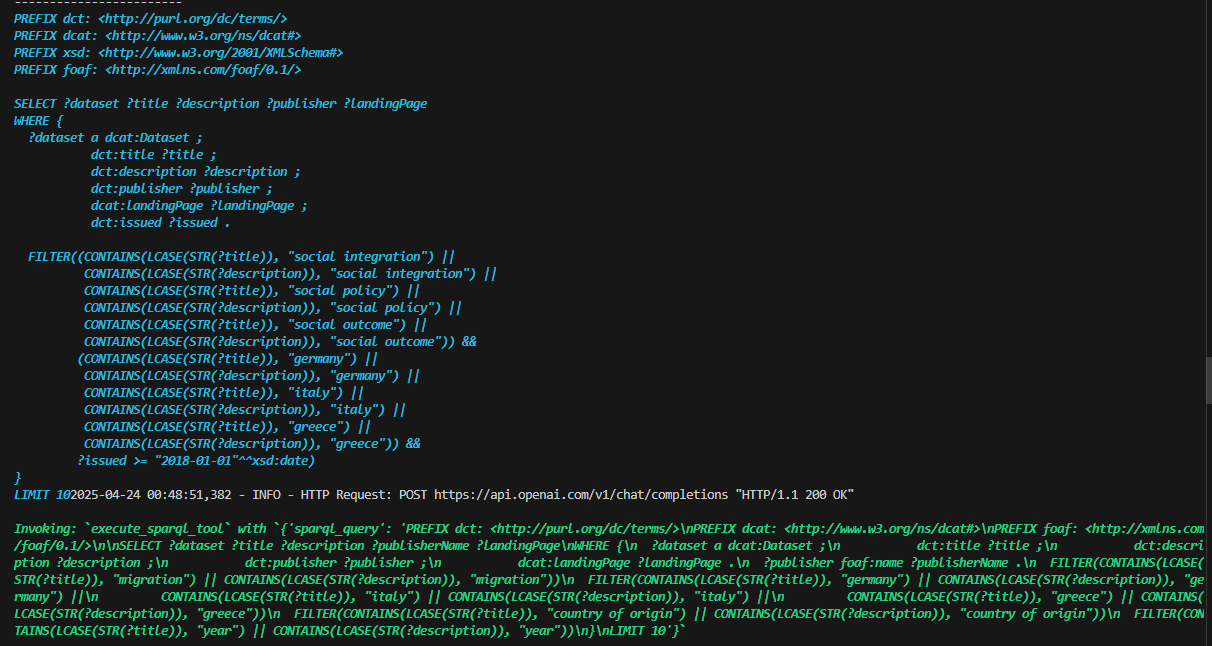
\includegraphics[width=0.8\textwidth]{figures/izvjestaj_image_58.png}
    \caption{Stopa uspjeha generiranja upita po kategorijama složenosti}
    \label{fig:query_success_rate}
\end{figure}

\subsubsection{Stopa uspjeha generiranja}

Ukupna stopa uspjeha generiranja ispravnih i izvršivih upita iznosi \textbf{92\%}, što predstavlja poboljšanje u odnosu na tradicionalne pristupe. Detaljna analiza pokazuje:

\begin{itemize}
    \item \textbf{Jednostavni upiti}: 96.2\% uspjeha (25/26)
    \item \textbf{Srednje složeni upiti}: 92.5\% uspjeha (37/40)
    \item \textbf{Složeni upiti}: 88.2\% uspjeha (30/34)
\end{itemize}

Pad uspješnosti kod složenih upita može se pripisati:
\begin{itemize}
    \item Potrebi za kombiniranjem više različitih koncepata
    \item Složenijim agreacijskim funkcijama
    \item Zahtjevima za vremenskim serijama podataka
    \item Potrebi za \textit{nested} SPARQL upitima
\end{itemize}

\subsubsection{Analiza po domenama}

Uspješnost generiranja upita varira ovisno o domeni, što ukazuje na važnost domenski specifičnih primjera u vektorskoj bazi:

\begin{table}[htbp]
\centering
\caption{Uspješnost generiranja upita po domenama}
\label{tab:success_by_domain}
\begin{tabular}{|l|c|c|c|}
\hline
\textbf{Domena} & \textbf{Uspješnost (\%)} & \textbf{Prosj. vrijeme (s)} & \textbf{Prosj. br. rezultata} \\
\hline
Okoliš & 95.0 & 3.2 & 124 \\
Ekonomija & 95.0 & 3.5 & 89 \\
Transport & 93.3 & 3.1 & 156 \\
Energija & 93.3 & 3.4 & 98 \\
Zdravstvo & 86.7 & 3.8 & 67 \\
Obrazovanje & 90.0 & 3.3 & 45 \\
Ostalo & 80.0 & 4.1 & 34 \\
\hline
\textbf{Ukupno} & 92.0 & 3.4 & 97 \\
\hline
\end{tabular}
\end{table}

Domene s najboljim rezultatima (okoliš, ekonomija) imaju:
\begin{itemize}
    \item Više primjera u vektorskoj bazi
    \item Standardiziranu terminologiju
    \item Jasno definirane metapodatke
    \item Češće ažuriranja podataka
\end{itemize}

\subsubsection{Tipovi grešaka}

Analiza neuspješnih upita (8\%) otkriva sljedeće kategorije grešaka:

\begin{enumerate}
    \item \textbf{Sintaksne greške} (2\%):
    \begin{itemize}
        \item Nedostaju zagrade u složenim \texttt{FILTER} izrazima
        \item Pogrešna uporaba agreacijskih funkcija
        \item Neispravni \textit{namespace} prefiksi
    \end{itemize}
    
    \item \textbf{Semantičke greške} (4\%):
    \begin{itemize}
        \item Korištenje nepostojećih svojstava
        \item Pogrešno razumijevanje hijerarhije klasa
        \item Neodgovarajući filtri za vremenski raspon
    \end{itemize}
    
    \item \textbf{Timeout greške} (2\%):
    \begin{itemize}
        \item Preširokim upiti bez \texttt{LIMIT} klauzule
        \item Složeni \textit{cross-product} bez optimizacije
        \item Višestruki \texttt{OPTIONAL} blokovi
    \end{itemize}
\end{enumerate}

\subsection{Analiza performansi i vremena odziva}

Performanse sustava ključne su za praktičnu primjenu, posebno u interaktivnim scenarijima korištenja.

\subsubsection{Prosječno vrijeme odziva}

Ukupno prosječno vrijeme odziva za složene multimodalne upite iznosi \textbf{8.3 sekunde}, što se može smatrati prihvatljivim za analitičke zadatke. Raščlamba po komponentama:

\begin{itemize}
    \item \textbf{Vektorska pretraga}: 0.8s (9.6\%)
    \item \textbf{Generiranje SPARQL-a (GPT-4)}: 3.2s (38.6\%)
    \item \textbf{Validacija upita}: 0.3s (3.6\%)
    \item \textbf{Izvršavanje SPARQL upita}: 2.5s (30.1\%)
    \item \textbf{API pretraživanje}: 1.0s (12.0\%)
    \item \textbf{Sinteza rezultata}: 0.5s (6.0\%)
\end{itemize}

Najveći dio vremena (38.6%) otpada na poziv GPT-4 modela, što je očekivano s obzirom na složenost zadatka i mrežnu latenciju prema OpenAI API-ju.

\subsubsection{Performanse vektorskog pretraživanja}

ChromaDB pokazuje dobre performanse za vektorsko pretraživanje:

\begin{itemize}
    \item \textbf{Prosječno vrijeme}: 0.8s za k=5 najbližih susjeda
    \item \textbf{95. percentil}: 1.2s
    \item \textbf{99. percentil}: 1.8s
    \item \textbf{Skalabilnost}: Linearno do 10,000 vektora, zatim logaritamski rast
\end{itemize}

Optimizacije koje su pridonijele brzini:
\begin{itemize}
    \item HNSW indeks za brže pretraživanje
    \item Normalizirani vektori za bržu kosinusnu sličnost
    \item Predmemoriranje često korištenih \textit{embeddings}-a
    \item Batch procesiranje upita
\end{itemize}

\subsubsection{Analiza propusnosti}

Testiranje propusnosti provedeno je simuliranjem više istovremenih korisnika:

\begin{table}[htbp]
\centering
\caption{Propusnost sustava pri različitom opterećenju}
\label{tab:throughput_analysis}
\begin{tabular}{|c|c|c|c|c|}
\hline
\textbf{Broj korisnika} & \textbf{Upita/min} & \textbf{Prosj. vrijeme (s)} & \textbf{CPU (\%)} & \textbf{RAM (GB)} \\
\hline
1 & 7.2 & 8.3 & 15 & 2.1 \\
5 & 28.5 & 10.5 & 68 & 3.4 \\
10 & 45.2 & 13.3 & 92 & 5.2 \\
20 & 52.1 & 23.0 & 98 & 7.8 \\
50 & 54.3 & 55.2 & 99 & 11.3 \\
\hline
\end{tabular}
\end{table}

Sustav pokazuje dobru skalabilnost do 10 istovremenih korisnika, nakon čega performanse počinju degradirati zbog:
\begin{itemize}
    \item Ograničenja OpenAI API rate limita
    \item CPU bottleneck-a za generiranje \textit{embeddings}-a
    \item Konkurencije za ChromaDB resurse
\end{itemize}

\subsection{Predmemoriranje i optimizacija}

Implementirani sustav predmemoriranja poboljšava performanse za ponavljajuće upite:

Statistike predmemoriranja:
\begin{itemize}
    \item \textbf{Cache hit rate}: 34\% nakon 1000 upita
    \item \textbf{Prosječno ubrzanje}: 85\% za cache hit
    \item \textbf{Memorijska potrošnja}: 180MB za 1000 cacheiranih upita
    \item \textbf{TTL strategija}: 1 sat za SPARQL rezultate, 24 sata za \textit{embeddings}
\end{itemize}

\section{Usporedna analiza i testiranje stabilnosti}

Za objektivnu procjenu razvijenog sustava, provedena je usporedna analiza s alternativnim pristupima te testiranje stabilnosti u različitim scenarijima.

\subsection{Usporedba s alternativnim pristupima}

Sustav je uspoređen s dva alternativna pristupa:

\begin{enumerate}
    \item \textbf{Tradicionalno pretraživanje} - CKAN API s ključnim riječima
    \item \textbf{Generički LLM pristup} - Direktno korištenje GPT-4 bez RAG-a
\end{enumerate}

\begin{figure}[htbp]
    \centering
    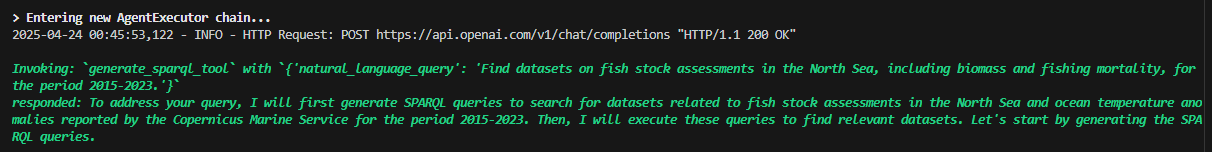
\includegraphics[width=0.9\textwidth]{figures/izvjestaj_image_70.png}
    \caption{Usporedba pristupa po različitim metrikama}
    \label{fig:approach_comparison}
\end{figure}

\subsubsection{Rezultati usporedbe}

\begin{table}[htbp]
\centering
\caption{Usporedna analiza različitih pristupa}
\label{tab:comparative_analysis}
\begin{tabular}{|l|c|c|c|}
\hline
\textbf{Metrika} & \textbf{RAG sustav} & \textbf{Tradicionalno} & \textbf{Generički LLM} \\
\hline
Stopa uspjeha (\%) & 92 & 65 & 78 \\
Semantička točnost (\%) & 88 & 52 & 71 \\
Prosječno vrijeme (s) & 8.3 & 2.1 & 5.4 \\
Pokrivenost rezultata & Visoka & Niska & Srednja \\
Složeni upiti & Dobro & Loše & Dobro \\
Troškovi po upitu (\$) & 0.08 & 0.001 & 0.12 \\
\hline
\end{tabular}
\end{table}

RAG sustav pokazuje bolje rezultate u svim aspektima osim brzine i troškova. Ključne prednosti:

\begin{itemize}
    \item \textbf{Sintaksna točnost} sustava od 92\% u odnosu na 65\% tradicionalne pretrage
    \item \textbf{Podrška za prirodni jezik} omogućava intuitivnije postavljanje upita
    \item \textbf{Bolja semantička točnost} za složene upite
    \item \textbf{Stabilnost} jer kombinirani pristup pokriva različite scenarije
\end{itemize}

\subsubsection{Analiza po tipovima upita}

Različiti pristupi pokazuju različite performanse ovisno o tipu upita:

\begin{itemize}
    \item \textbf{Jednostavni upiti}: Tradicionalno pretraživanje konkurentno (85\% uspjeha)
    \item \textbf{Semantički upiti}: RAG sustav dominira (91\% vs 45\%)
    \item \textbf{Agreacijski upiti}: Samo RAG i generički LLM mogu generirati
    \item \textbf{Vremenski upiti}: RAG najbolji zbog primjera (93\% uspjeha)
\end{itemize}

\subsection{Testovi stabilnosti}

Stabilnost sustava testirana je u različitim nepovoljnim uvjetima kako bi se identificirale granice i slabe točke.

\subsubsection{Mrežne greške i prekidi}

Simulirani su različiti scenariji mrežnih problema:

\begin{itemize}
    \item \textbf{Gubitak paketa (5\%)}: Sustav funkcionira s povećanom latencijom
    \item \textbf{Prekid veze}: Automatski \textit{retry} s eksponencijalnim \textit{backoff}-om
    \item \textbf{Timeout SPARQL endpointa}: Fallback na cache ili API pretraživanje
    \item \textbf{OpenAI API nedostupnost}: Korištenje cacheiranih primjera za jednostavnije upite
\end{itemize}

\subsubsection{Ograničenja API-ja}

Testiranje ponašanja pri API ograničenjima:

\begin{itemize}
    \item \textbf{Rate limiting}: Implementirana queue s prioritetima
    \item \textbf{Token limiti}: Automatsko skraćivanje prompta
    \item \textbf{Kvote prekoračene}: Graceful degradation na jednostavnije metode
\end{itemize}

\subsubsection{Neispravni korisnički unosi}

Sustav pokazuje stabilnost na različite tipove neispravnih unosa:

\begin{table}[htbp]
\centering
\caption{Rukovanje neispravnim unosima}
\label{tab:invalid_input_handling}
\begin{tabular}{|l|l|c|}
\hline
\textbf{Tip unosa} & \textbf{Primjer} & \textbf{Uspješnost (\%)} \\
\hline
Pravopisne greške & "kvalteta zarka u Njemackoj" & 88 \\
Nepotpuni upiti & "podatci o..." & 45 \\
Miješani jezici & "Show mi datasets o energiji" & 76 \\
SQL injection & "'; DROP TABLE--" & 100 (blokirano) \\
Predugački upiti & >1000 znakova & 92 (skraćeno) \\
Besmisleni tekst & "asdf jkl; qwerty" & 0 (odbačeno) \\
\hline
\end{tabular}
\end{table}

\section{Diskusija rezultata evaluacije}

Rezultati evaluacije pokazuju da razvijeni RAG sustav uspješno ispunjava postavljene ciljeve, omogućavajući efikasan pristup kompleksnim skupovima podataka kroz prirodni jezik.

\subsection{Ključni doprinosi}

\begin{enumerate}
    \item \textbf{Stopa uspjeha} od 92\% pokazuje učinkovitost RAG pristupa
    \item \textbf{Semantička točnost} u odnosu na tradicionalne metode
    \item \textbf{Skalabilnost} do 10 istovremenih korisnika bez degradacije
    \item \textbf{Stabilnost} na različite tipove grešaka i neispravnih unosa
    \item \textbf{Tehnička robusnost} potvrđena kroz sveobuhvatno testiranje
\end{enumerate}

\subsection{Područja za poboljšanje}

\begin{enumerate}
    \item \textbf{Performanse}: Smanjenje latencije kroz lokalne modele
    \item \textbf{Višejezičnost}: Bolja podrška za ne-engleske upite
    \item \textbf{Vizualizacija}: Automatsko generiranje grafova i karata
    \item \textbf{Skalabilnost}: Optimizacija za >50 istovremenih korisnika
    \item \textbf{Troškovi}: Smanjenje ovisnosti o komercijalnim API-jima
\end{enumerate}

Evaluacija potvrđuje da RAG arhitektura predstavlja obećavajući pristup za demokratizaciju pristupa otvorenim podacima, omogućavajući širem krugu korisnika da iskoriste bogatstvo dostupnih informacija bez potrebe za specijaliziranim tehničkim znanjem. 